\section{Сферическая астрономия}

Раздел сферической астрономии или небесной сферы собирает в себе темы, связанные с положением и движением небесных тел по небесной сфере в результате суточного и годичного движение Земли. Для дальнейшего повествования определим некоторые термины, на которых оно будет построено.

\term{Большой круг сферы}~--- окружность на поверхности сферы, центр которого совпадает с центром сферы.

Здесь и далее \imp{осью вращения} будем называть неподвижную ось вращения сферы, проходящую через ее центр. 

\term{Экватор}~--- большой круг, перпендикулярный оси вращения. Точки пересечения оси вращения со сферой называются \term{полюсами}.

\term{Малый круг сферы}~--- произвольная окружность на поверхности сферы. \term{Параллель}~--- малый круг, параллельный экватору.

Большой круг, перпендикулярный экватору, называется \term{мери\-диа\-ном}. Угловое расстояние между заданной точкой $A$ и точкой пересечения меридиана, проходящего через точку $A$, с экватором называется \term{широтой} точки $A$. Широта обозначается греческой буквой $\varphi$. В северном полушарии $\varphi > 0$, в южном~--- $\varphi < 0$. Очевидно, $\varphi \in [-90; 90]$. \term{Полярное расстояние}~$p$~--- угловое расстояние между рассматриваемой точкой и точкой северного полюса. $p + \varphi = 90^\circ$.

Теперь можно перейти от геометрии к астрономии. 

\term{Наблюдатель}~--- материальная точка на поверхности сферы (Земли). \term{Небесная сфера}~--- воображаемая сфера произвольного (бесконечного) радиуса с центром в наблюдателе. \term{Точка небесной сферы}~--- воображаемая точка на небесной сфере, на самом деле являющаяся некоторым лучом с заданным направлением.

\term{Математический горизонт}~--- касательная плоскость к поверхности сферы в наблюдателе. Чаще математическим горизонтом называют большой круг небесной сферы~--- пересечение вышеописанной плоскости с небесной сферы. 

\term{Зенит}~$Z$~--- (точка небесной сферы) луч, исходящий из наблюдателя от, перпендикулярный математическому горизонту, направлен от центра сферы. эквивалентично определяется точка \term{надира}~$Z'$, противоположная точке зенита.

\term{Полярная ось}~--- ось вращения небесной сферы, параллельная оси вращения Земли. \term{Полюс мира} (северный)~$P$~--- точка пересечения полярной оси с небесной сферой со стороны северного полюса Земли. Южный \imp{полюс мира}~$P'$~--- точка, противоположная северному полюсу мира.

Здесь возникает проблема: Земля вращается, а значит наблюдатель движется, и небесная небесная сфера смещается. То есть положения на небесной сфере неподвижных в пространстве звезд меняются. Это называется параллаксом, а котором говорилось в Разделе ??. 

В силу малости горизонтального параллакса можно сделать вывод, что для далеких небесных объектов можно им пренебречь и считать их неподвижными. Также в большинстве задач сферической астрономии пренебрегают и годичным параллаксом, хотя его величина уже не исчезающе мала. 

Однако из этого всего не следует, что нужно совсем забывать про явления параллакса. Важно при решении каждой задачи на сферическую астрономию проверять необходимость учета этого явления.

Так или иначе, пренебрегая размером Земли, можно считать, что наблюдатель находится в центре Земли. А плоскостью математического горизонта, все также проходит через наблюдателя и параллельна изначальной.

\term{Небесный экватор}~--- большой круг небесной сферы, перпендикулярный полярной оси. \term{Суточная параллель}~--- путь неподвижного небесного объекта в течение суток по небесной сфере, является малым кругом, эквивалент~--- параллель.

\term{Север}~$N$ и \term{юг}~$S$~--- точки небесной сферы на математическом горизонте, лежащие на одном луче с проекциями соответствующих полюсов мира на математический горизонт.

Нетрудно показать, что точки $P$~--- северный полюс мира, $P'$~--- южный полюс мира, $Z$~--- зенит, $Z'$~--- надир, $N$~--- север и $S$~---юг лежат на одном большом круге. Этот круг называется \term{небесным меридианом}.


\subsection{Системы небесных координат}
Каждая из систем небесных координат является сферической системой координат, в которой радиус не имеет значения, так как параллакс не учитывается, а объекты считаются бесконечно удалёнными от наблюдателя.

\begin{figure}[!h]
	\centering
	\begin{subcaptionblock}{0.49\textwidth}
		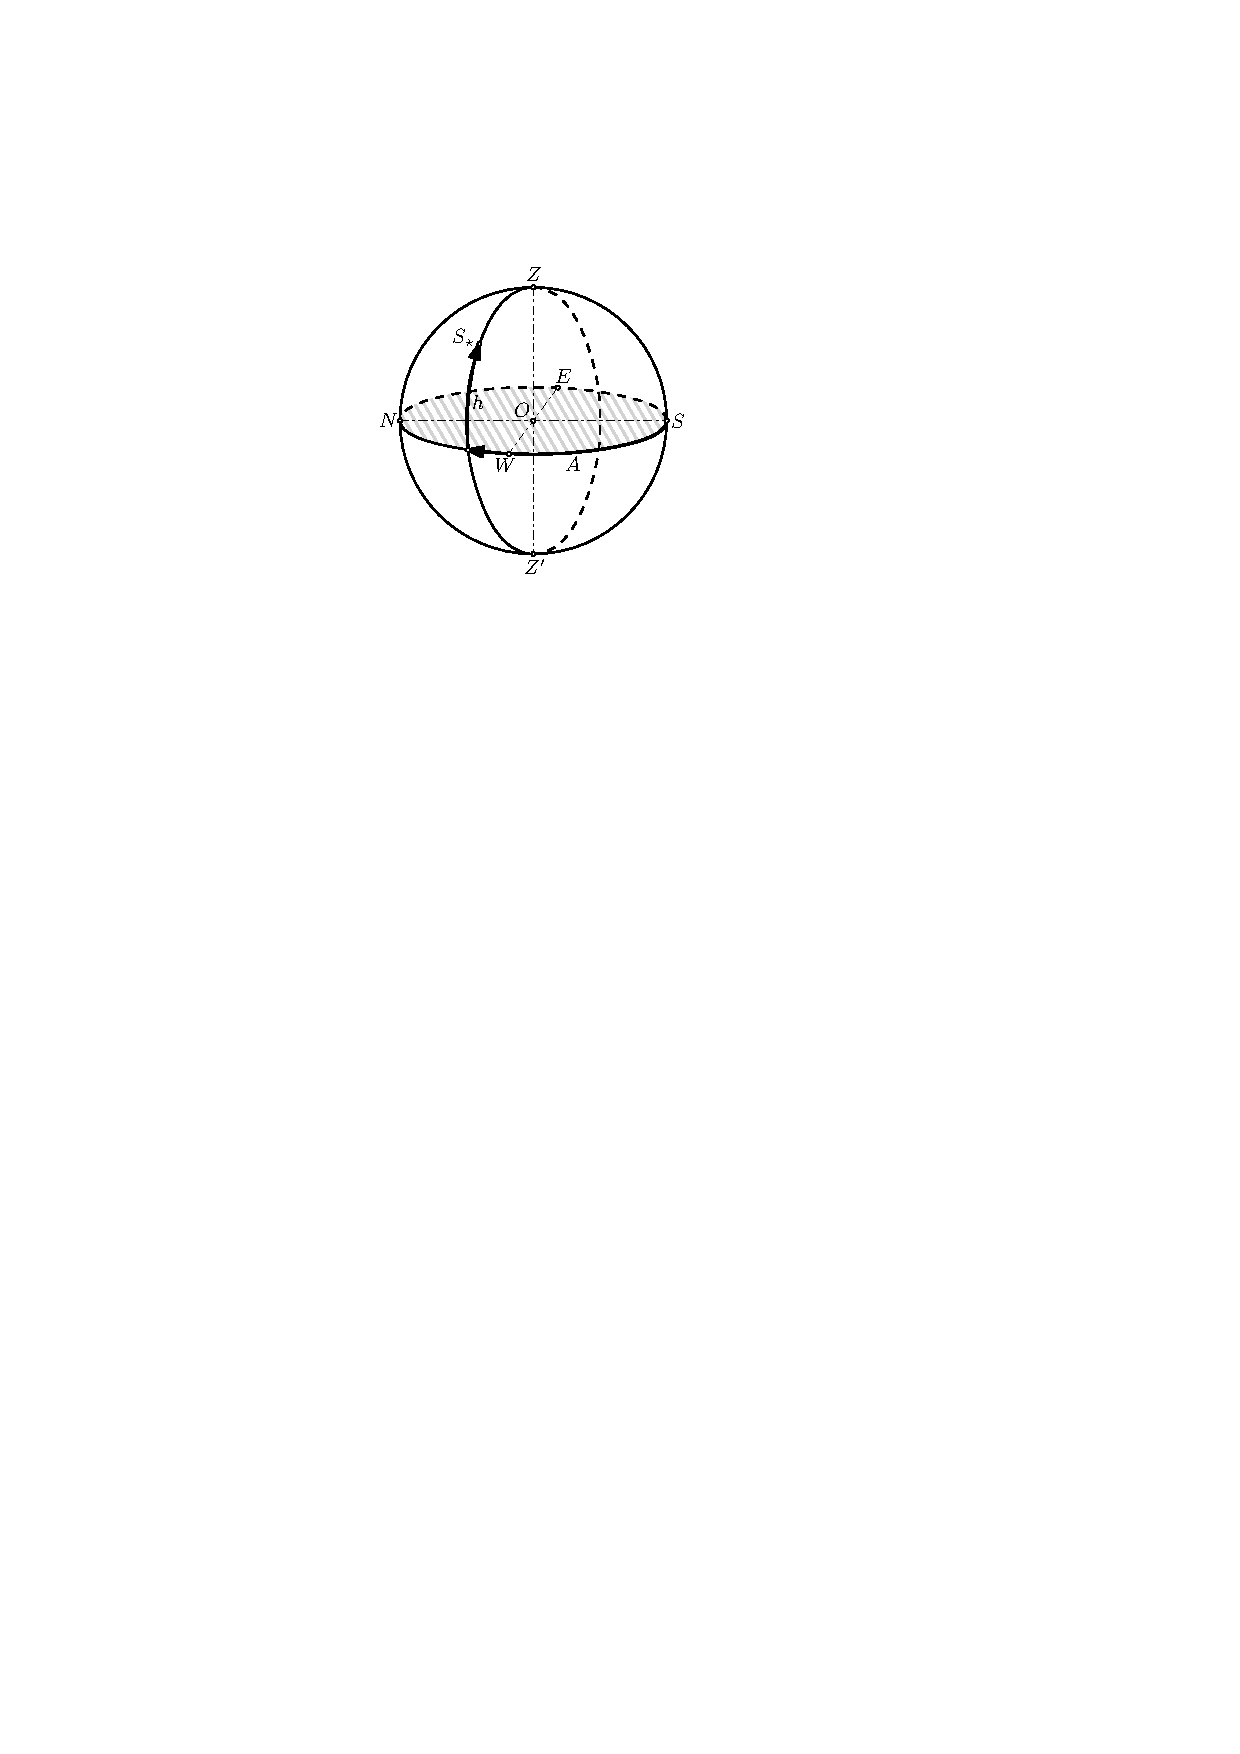
\includegraphics[width = \textwidth]{hor-coordin-sys}
		\caption{Горизонтальная система координат}
	\end{subcaptionblock}
	\hfill
	\begin{subcaptionblock}{0.49\textwidth}
		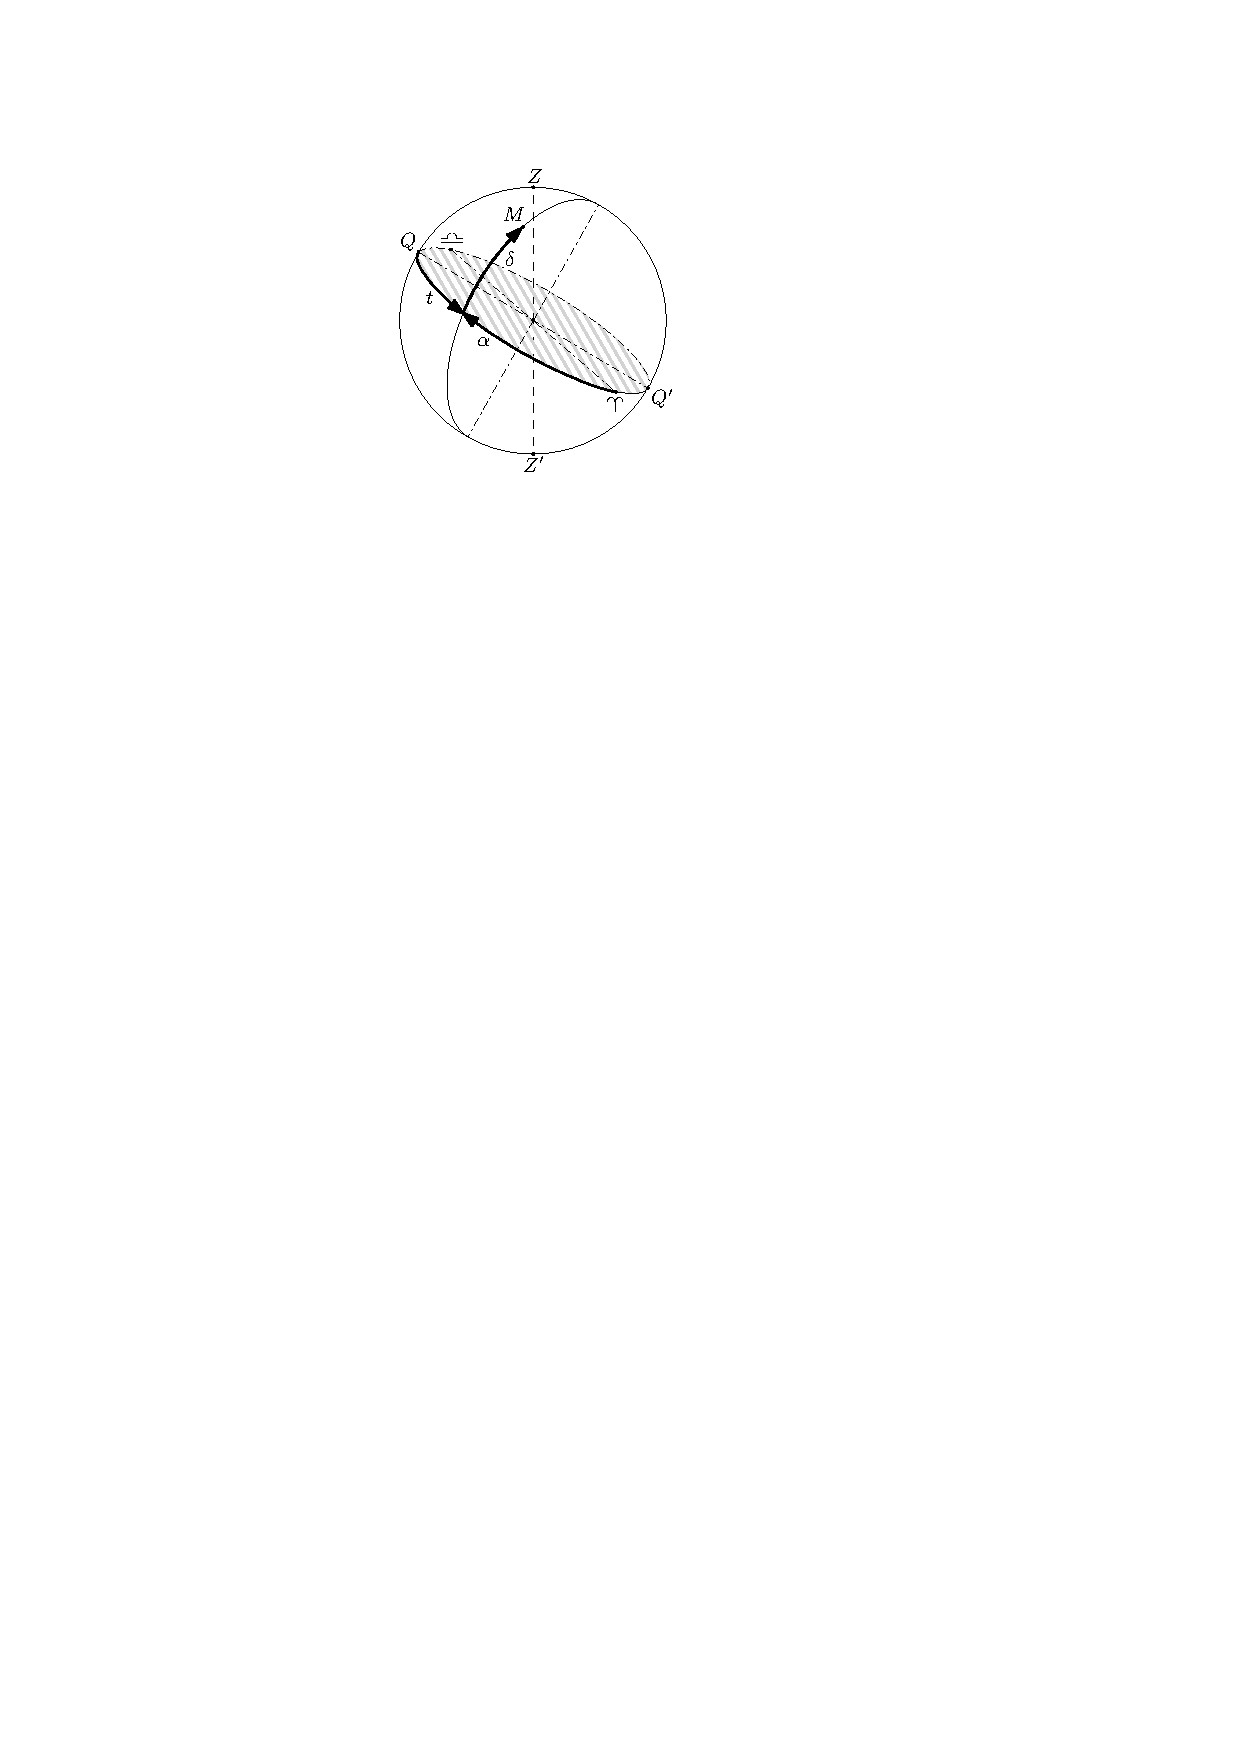
\includegraphics[width = \textwidth]{eq-coordin-sys}
		\caption{Экваториальная система координат}
	\end{subcaptionblock}
	\caption{Системы координат I}
\end{figure}
\term{Горизонтальная система координат}~--- система координат, в которой основной плоскостью является плоскость математического горизонта, а полюсами~--- \term{зенит} и \term{надир}~--- точки небесной сферы, расположенные ровно над наблюдателем и под ним соответственно. Одной координатой является либо \term{высота} светила $h$~--- угловое расстояние между светилом и математическим горизонтом, отсчитываемое в сторону зенита, либо его \term{зенитное расстояние}~$z$~--- угловое расстояние между зенитом и светилом. Другой координатой является \term{астрономический азимут} $A$~--- угол $SZS_\star$, отсчитываемый в сторону запада. Половина большого круга, перпендикулярного горизонту,~--- $Z S_\star Z'$  называется \term{вертикалом} объекта.

\term[экваториальная система координат]{Первая экваториальная система координат}~--- система координат,
основной плоскостью которой является плоскость небесного экватора $QEQW'$.
Одной координатой при этом является \term{склонение}~$\delta$~--- угловое
расстояние между светилом и плоскостью небесного экватора, отсчитываемое в
сторону севера. Половина большого круга, вдоль которой отсчитывается склонение,
перпендикулярна небесному экватору и называется \term[круг склонений]{кругом склонений} или
\imp{кругом равных часовых углов (прямых восхождений)}. Наряду со склонением
используется \term{полярное расстояние}~$p$~--- угловое расстояние между
светилом и полюсом мира. Другой координатой является \term{часовой угол}~$t$~---
дуга небесного экватора от верхней точки небесного экватора до круга склонения
светила в сторону запада, или угол между небесным меридианом и кругом склонения
светила. $\aries$ и $\libra$~--- точки весеннего и осеннего равноденствия соответственно.

\term[экваториальная система координат]{Вторая экваториальная система координат}~--- система, аналогичная предыдущей. Одной координатой по прежнему является \term{склонение}~$\delta$. А другой координатой является \term{прямое восхождение}~$\alpha$~--- угловое расстояние между точкой весеннего равноденствия и кругом склонений светила в сторону годичного движения Солнца.

\begin{figure}[!h]
	\centering
	\begin{subcaptionblock}{0.49\textwidth}
		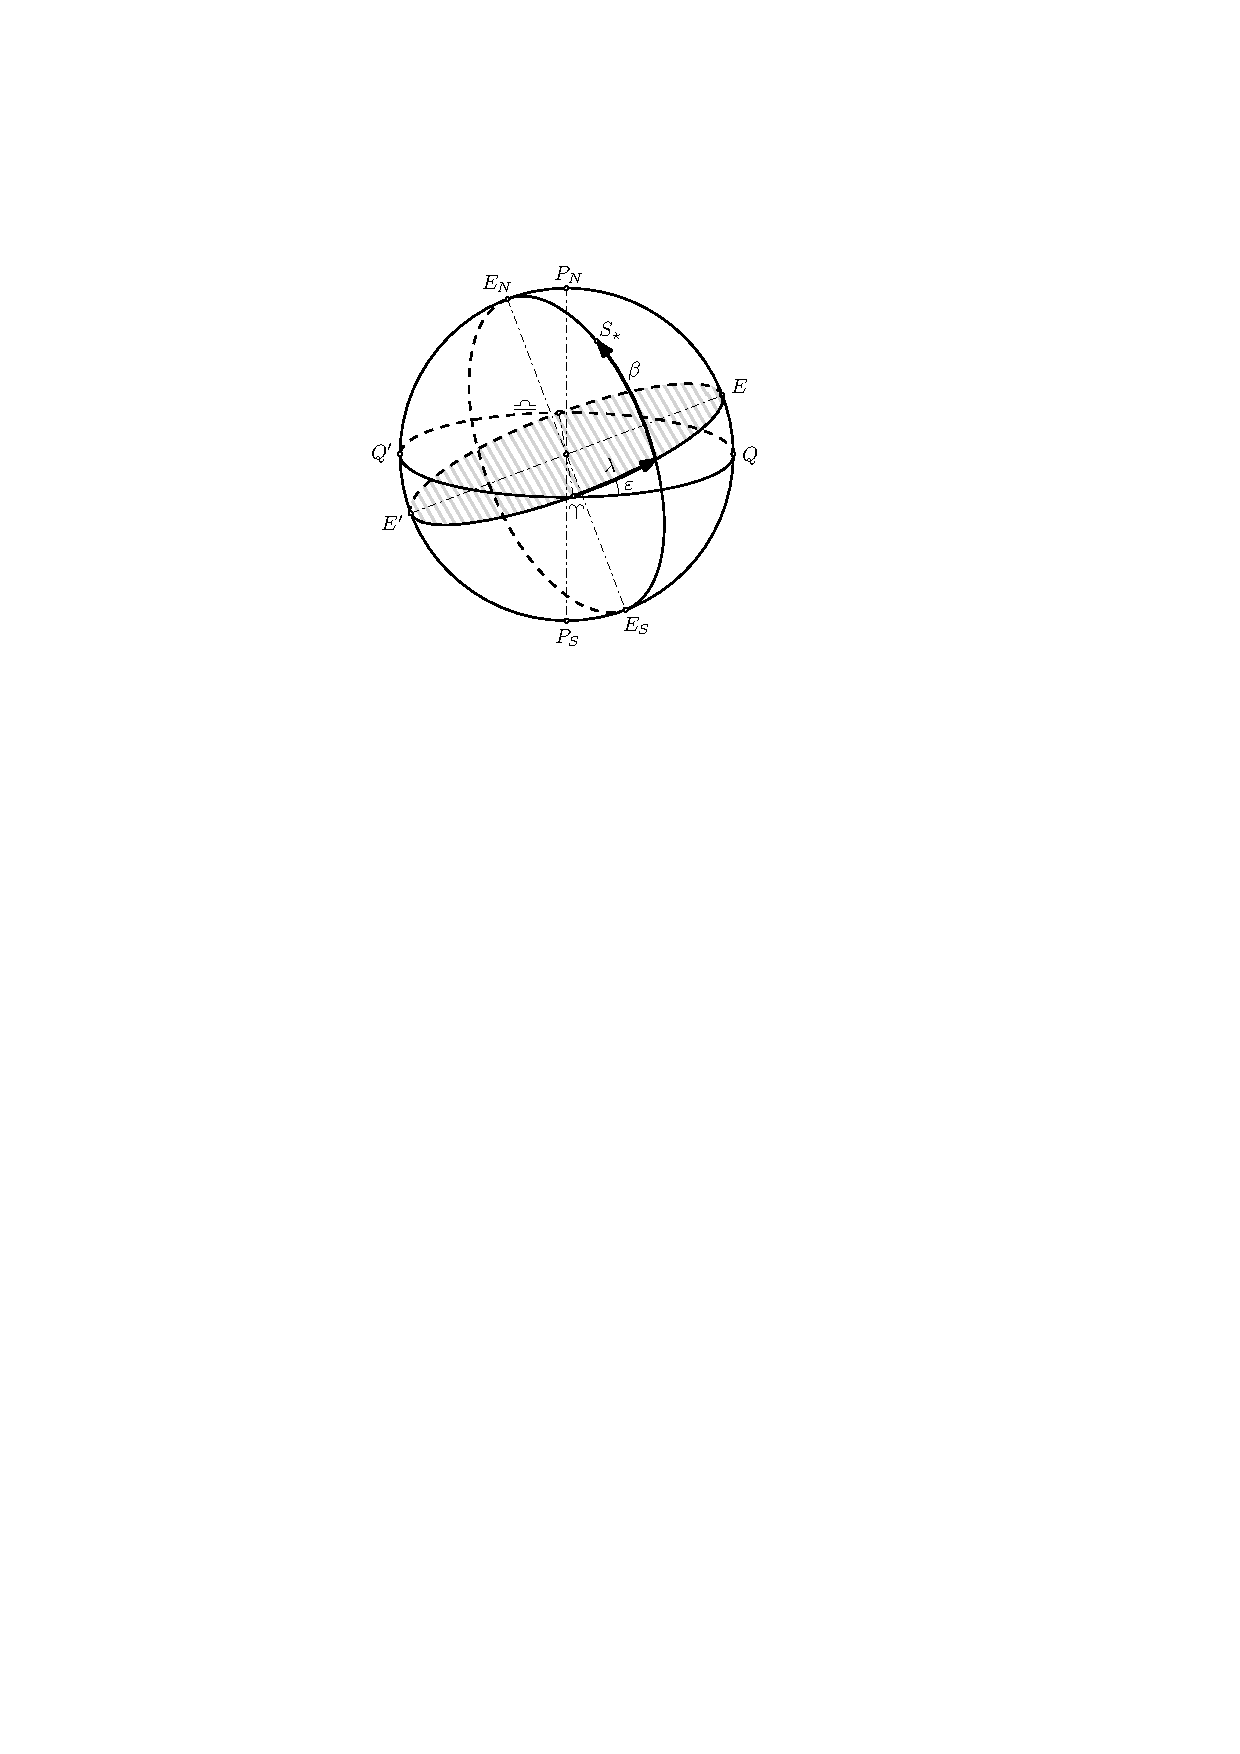
\includegraphics[width = \textwidth]{eql-coordin-sys}
		\caption{Эклиптическая система координат}
	\end{subcaptionblock}
	\hfill
	\begin{subcaptionblock}{0.49\textwidth}
		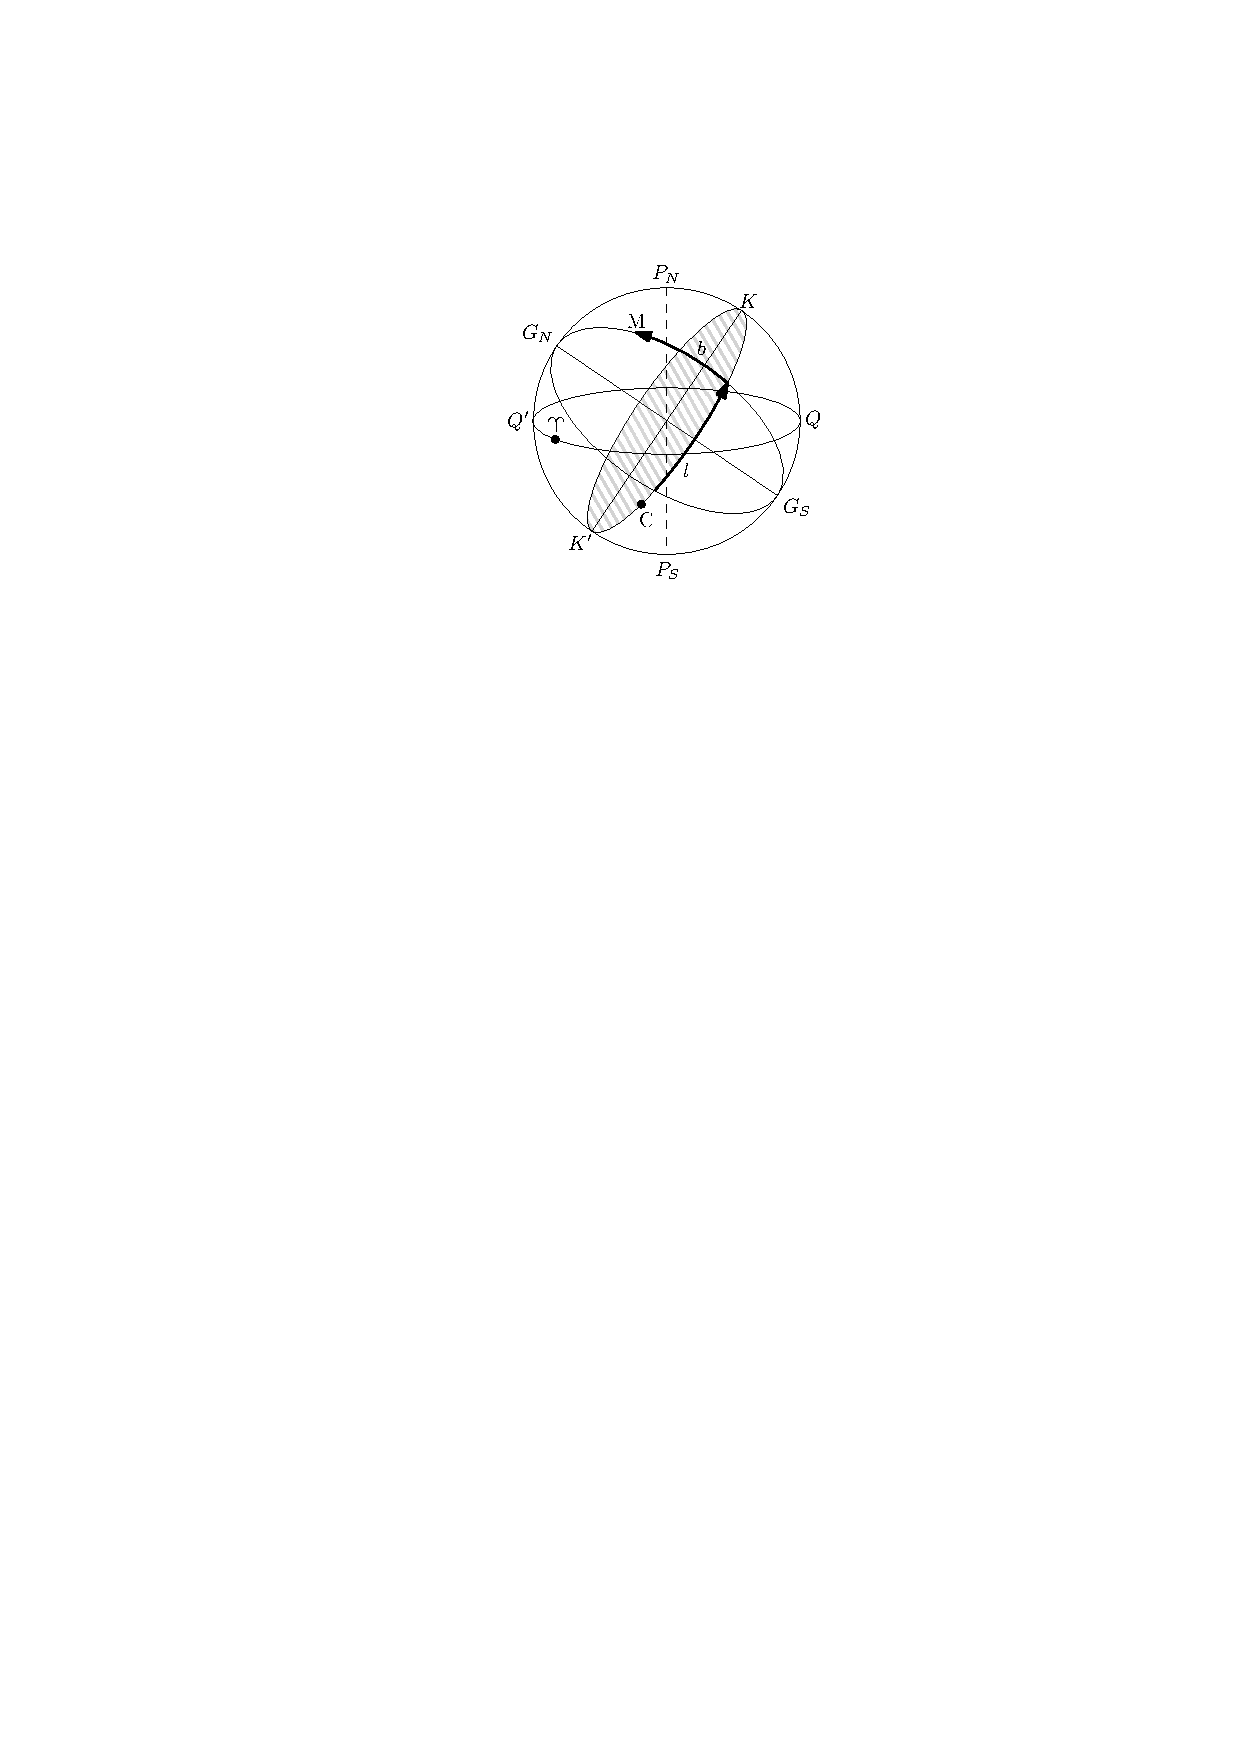
\includegraphics[width = \textwidth]{gal-coordin-sys}
		\caption{Галактическая система координат}
	\end{subcaptionblock}
	\caption{Системы координат II}
\end{figure}
\term{Эклиптическая система координат}~--- система координат, основной плоскостью которой является плоскость эклиптики $E \libra E' \aries $. Одной координатой при этом является \term{эклиптическая широта}~$\beta$~--- угловое расстояние между светилом и плоскостью эклиптики, отсчитываемое в сторону северного полюса мира, а другой~--- \term{эклиптическая долгота}~$\lambda$~--- угловое расстояние между точкой весеннего равноденствия и кругом эклиптической широты светила. Полюса эклиптики $E_N$ и $E_S$ имеют координаты ($18^h$,~$90^\circ - \varepsilon$) и ($6^h$,~$-90^\circ + \varepsilon$).

\term{Галактическая система координат}~--- система координат, основной плоскостью которой является плоскость нашей галактики, которая наклонена к плоскости небесного экватора под углом $62.6^\circ$. Одной координатой при этом является \term{галактическая широта}~$b$~--- угол между плоскостью галактического экватора и направлением на светило, а другой~--- \term{галактическая долгота}~$l$~--- угол между направлением на точку начала отсчёта $C$ и плоскостью круга галактической широты светила. Точка $C$ является направлением на центр галактики и имеет координаты: $\alpha=17^h\,45.6^m$, $\delta=-28^{\circ}\,56.2'$. $C K K'$~--- плоскость галактического экватора; $G_N$, $G_S$~--- северный и южный полюса галактики соответственно.

\subsection{Суточное вращение небесной сферы}
Вследствие вращения Земли вокруг своей оси для наблюдателя на поверхности небесные объекты совершают суточное движение параллельно небесному экватору, плоскость которого совпадает с плоскостью экватора Земли. Очевидно, в ходе такого движения высота светил постоянно меняется и в некоторые моменты времени достигает своего максимального и минимального значения.

\term[верхняя кульминация]{Верхняя} и \term{нижняя кульминация}~--- моменты пересечения светилом небесного меридиана, причём при верхней кульминации светило имеет наибольшую высоту, а при нижней~--- наименьшую.

Высота светила в верхней и нижней кульминации со склонением $|\delta| < |\varphi|$, соответственно:
\begin{equation}
	h_{\text{в}}= 90^\circ - \varphi + \delta, \quad\quad
	h_{\text{н}}= - 90^\circ + \varphi  + \delta.
\end{equation}

Если же светило имеет склонение $|\delta| > |\varphi|$, то высота в верхней и нижней кульминации вычисляется так:
\begin{equation}
	h_{\text{в}}= 90^\circ + \varphi - \delta, \quad\quad
	h_{\text{н}}= - 90^\circ -\varphi - \delta.
\end{equation}

Из формул для высоты в нижней кульминации вытекает условие, определяющее, пересекает ли звезда горизонт:
\begin{equation}
	\begin{cases}
		h_\text{в} = +90^\circ - |\varphi - \delta| > 0^\circ,\\
		h_\text{н} = - 90^\circ + |\varphi + \delta| < 0^\circ;
	\end{cases}
	\quad \Longleftrightarrow \quad~~ |\delta|< 90^{\circ} - |\varphi|.
\end{equation}

Используя формулы сферической тригонометрии (см.\,\ref{sec:spher-trig}), можно выразить зависимость часового угла светила от его зенитного расстояния:
\begin{equation}
	\cos t=\frac{\cos z-\sin\varphi\sin\delta}{\cos\varphi\cos\delta}.
\end{equation}
Отсюда следует, что для часового угла захода и восхода светила справедливо равенство:
\begin{equation}
	\cos t_{\uparrow\downarrow}=-\tg\varphi\cdot\tg\delta.
\end{equation}

Аналогично, для вычисления азимута светила верна формула
\begin{equation}
	\cos A=\frac{\cos\delta\cos t-\cos\varphi\cos z}{\sin\varphi\sin z}.
\end{equation}
Следовательно, азимуты точек восхода и захода
\begin{equation}
	A_\uparrow = \arccos \left(-\dfrac{\sin\delta}{\cos \varphi} \right)\quad\text{и}\quad A_\downarrow = - A_\uparrow.
\end{equation}

\term{Звёздное время}~$z$~--- часовой угол точки весеннего равноденствия. Из определений прямого восхождения и часового угла следует справедливость равенства\begin{equation}
z = \alpha + t.
\end{equation}

\subsection{Сферическая тригонометрия}
\label{sec:spher-trig}
\begin{wrapfigure}[10]{r}{.3\tw}
    \centering
    \vspace{-1pc}
    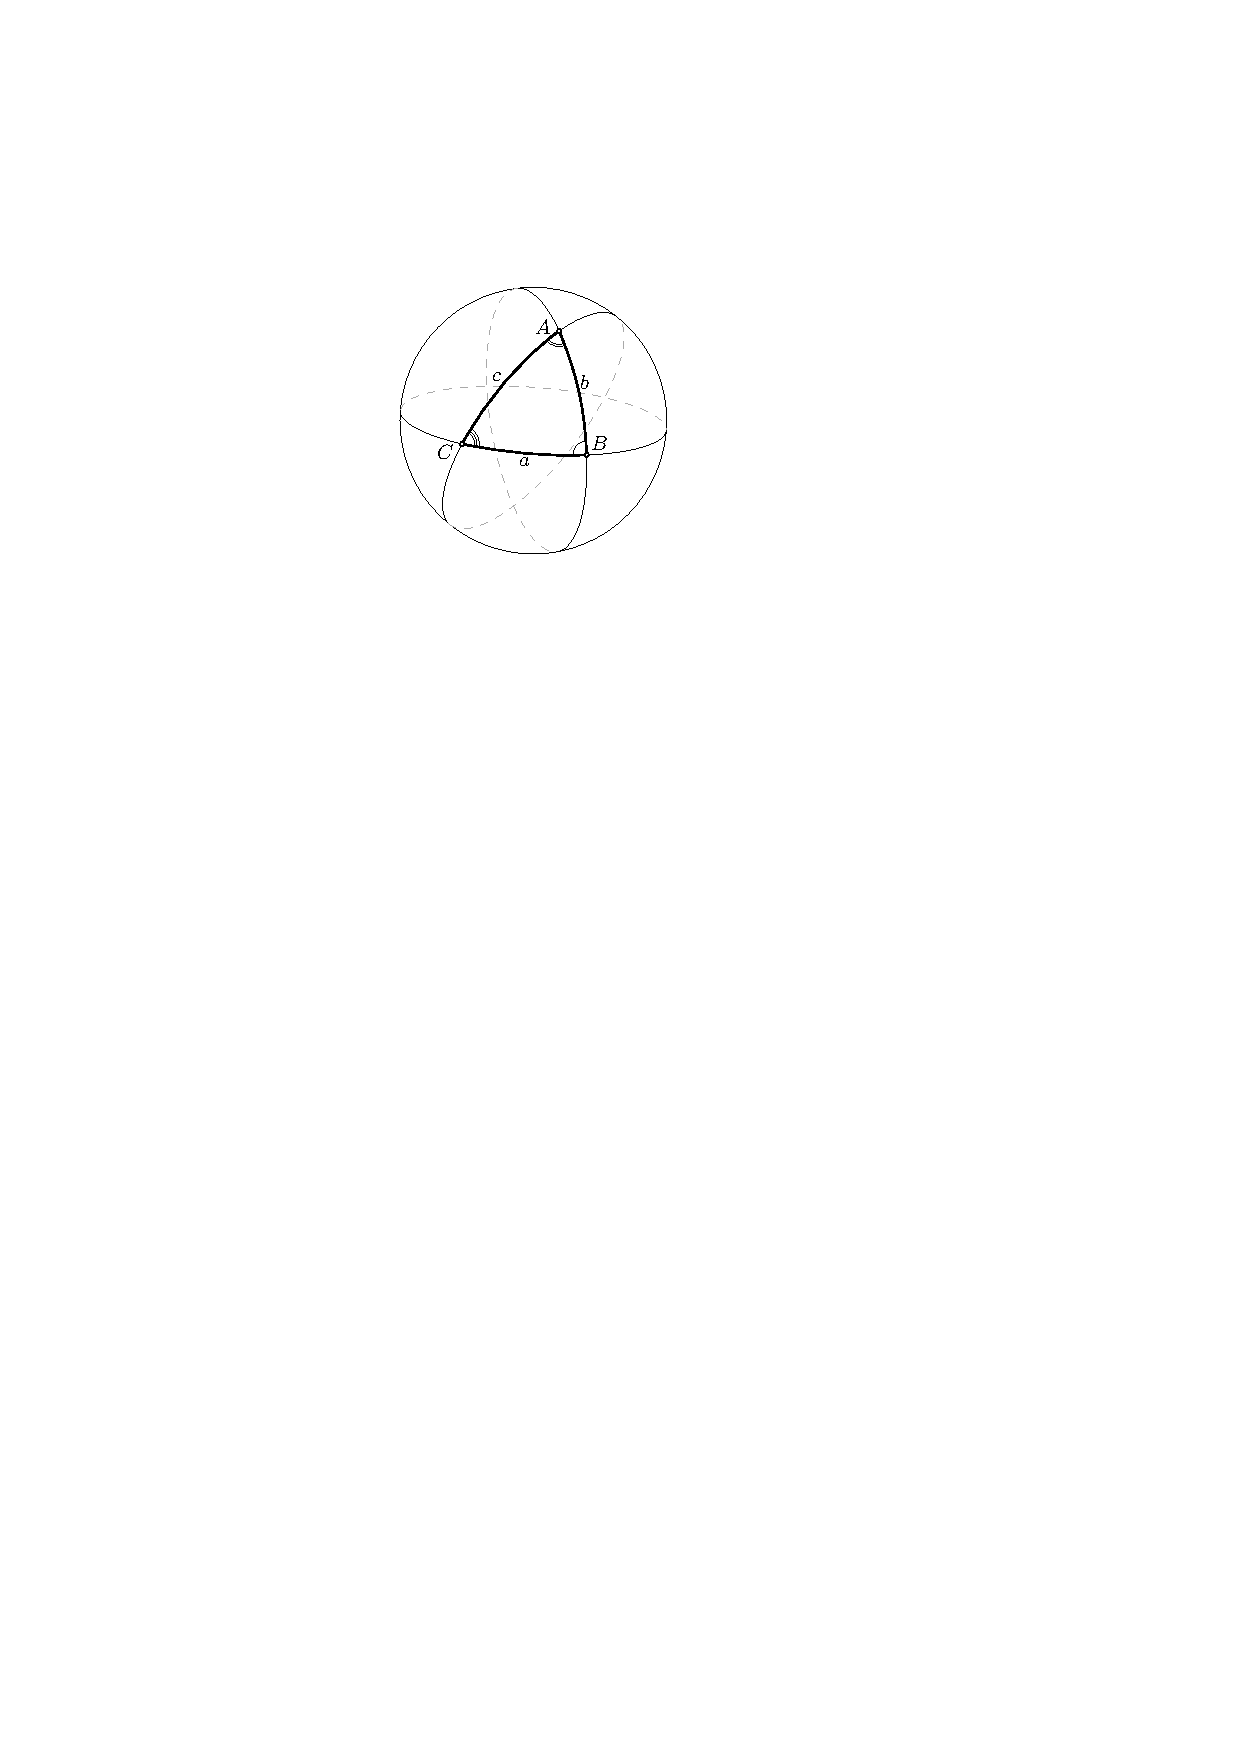
\includegraphics[width=0.3\textwidth]{spher-trigonom}
    \caption{Сферический треугольник}
\end{wrapfigure}
Для решения некоторых задач астрономии, связанных с видимыми положениями небесных тел, требуются знания о сферической тригонометрии. \imp{Сферический треугольник}~--- фигура на поверхности сферы, состоящая из трёх точек и трёх дуг больших кругов, соединяющих эти точки. Пусть $A$, $B$ и $C$~--- углы сферического треугольника, а $a$, $b$ и $c$~--- его стороны.

Сферические треугольники обладают следующими свойствами:
\begin{enumerate}
    \item Два сферических треугольника равны, если они подобны.
    \item Каждая сторона меньше суммы двух других сторон и больше их разности.
    \item Сумма всех сторон $a+b+c$ всегда меньше $2\pi$.
    \item Сумма углов сферического треугольника $\pi < A + B + C < 3\pi$.
    \item Разность суммы двух углов и третьего угла меньше $\pi$
\end{enumerate}

Площадь сферического треугольника определяется по формуле:
\begin{equation}
    S = R^2( A + B + C - \pi),
\end{equation}
где $A + B + C - \pi$~--- \imp{сферический избыток}.

Рассмотрим сферический треугольник $ABC$, радиус векторы вершин соответственно $\vec{a}$, $\vec{b}$ и $\vec{c}$.Причем из определения сферы $|\vec{a}| = |\vec{b}| = |\vec{c}| = r$. Пусть против вершин $A$, $B$ и $C$ лежат стороны с угловой мерой $a$, $b$ и $c$ соответсвенно. Повернем сферические координаты и нормируем так, чтобы $\vec{a} = (0, 0, 1)$, $\vec{b} = (\sin c, 0, \cos c)$, тогда $ \vec{c} = (\sin b \cos A, \sin b \sin A, \cos b)$.

Теперь запишем выражение для $\scalar{b}{c}$:
\begin{equation}
    \scalar{b}{c} = \cos a = \sin c \sin b \cos A + \cos c \cos b.
    \label{eq:spher-astro-cos-1}
\end{equation}
Аналогично,
\begin{gather}
    \scalar{a}{c} = \cos b = \sin a \sin c \cos B +  \cos a \cos c,\\
    \scalar{a}{b} = \cos c = \sin a \sin b \cos C + \cos a \cos b.
    \label{eq:spher-astro-cos-1-1}
\end{gather}
Выразим отсюда $\cos A$:
\begin{equation}
    \cos A = \frac{\cos a - \cos c \cos b}{\sin c \sin b}.
    \label{eq:spher-astro-cos-2}
\end{equation}
Формулы \eqref{eq:spher-astro-cos-1}\,--\,\eqref{eq:spher-astro-cos-2} называются \term{сферической теоремой косинусов} \imp{для стороны} \eqref{eq:spher-astro-cos-1}\,--\,\eqref{eq:spher-astro-cos-1-1} и, соответственно \imp{для угла} \eqref{eq:spher-astro-cos-2}.

Из основного тригонометрического тождества имеем:
\begin{multline*}
    \sin^2 A = 1 - \cos^2 A = 1 - \left[ \frac{\cos a - \cos c \cos b}{\sin c \sin b} \right]^2 = \\
    = \frac{\sin^2 c \sin^2 b - \cos^2 a + 2\cos a \cos c \cos b - \cos^2 c \cos^2 b}{\sin^2 c \sin^2 b}=\\
    = \frac{(1 - \cos^2 c)(1 -  \cos^2 b) - \cos^2 a + 2\cos a \cos c \cos b - \cos^2 c \cos^2 b}{\sin^2 c \sin^2 b}=\\
    = \frac{1 - \cos^2 c - \cos^2 b + \cos^2 c \cos^2 b -\cos^2 a}{\sin^2 c \sin^2 b} + \\
    + \frac{2\cos a \cos c \cos b - \cos^2 c \cos^2 b}{\sin^2 c \sin^2 b} = \\
    = \frac{1 - \cos^2 c - \cos^2 b - \cos^2 a + 2\cos a \cos c \cos b}{\sin^2 c \sin^2 b}.
\end{multline*}
Извлекая квадратный корень из левой и правой части и деля их на $\sin a$ имеем
\begin{equation*}
    \frac{\sin{A}}{\sin a} = \frac{\sqrt{1 - \cos^2 c - \cos^2 b - \cos^2 a + 2\cos a \cos c \cos b}}{\sin a \sin b \sin c}.
\end{equation*}
Заметим, что правая часть равенства циклична по переменным $a$, $b$ и $c$, следовательно, \term{сферическая теорема синусов} имеет вид
\begin{equation}
    \frac{\sin A}{\sin a} = \frac{\sin B}{\sin b} = \frac{\sin C}{\sin c}.
    \label{eq:sphere-th-sinus}
\end{equation}

Далее получим \term{формулу пяти элементов}. Для этого запишем теорему косинусов в выразим в ней один из косинусов, применяя ее же:
\begin{gather}
    \cos a = \sin c \sin b \cos A + \cos c \cos b,\nonumber\\
    \cos a = \sin c \sin b \cos A + \left( \sin a \sin b \cos C + \cos a \cos b \right)\cos b,\nonumber\\
    \cos a - \cos a \cos^2 b = \sin c \sin b \cos A + \sin a \sin b \cos b \cos C,\nonumber\\
    \cos a \sin^2 b = \sin c \sin b \cos A + \sin a \sin b \cos b \cos C,\nonumber\\
    \cos a \sin b = \sin a \cos b \cos C + \sin c \cos A.
    \label{eq:formula-5-elem}
\end{gather}


\begin{wrapfigure}[14]{r}{0.5\tw}
    \centering
    \vspace{-1pc}
    \tikzsetnextfilename{navigation-triangle}
    \tdplotsetmaincoords{70}{170}
    \begin{tikzpicture}[tdplot_main_coords]
        \footnotesize
        
        \def\r{2.5}
        \def\f{55}
        \def\d{20}
        \def\l{100}
        \def\t{60}


        % Draw spherical grid
        \draw[tdplot_screen_coords,thin,black!30] (0,0,0) circle (\r);
        \foreach \a in {-60,-30,...,60}{
            \tdplotCsDrawLatCircle[thin,black!20]{\r}{\a}
        }
        \foreach \a in {0,30,...,150}{
            \tdplotCsDrawLonCircle[thin,black!20]{\r}{\a}
        }
    
        
        % Delta coord of the intersection horizon and circle of equal right ascention
        \pgfmathsetmacro{\deltaMin}{atan(-cos(\t)/tan(\f))}
        
        % Angle between horizon and circle of equal right ascention
        \pgfmathsetmacro{\rotateAngle}{asin(cos(\t) * cos(\f) / sin(\deltaMin))}
        
        % 90 - Azimuth coord of the intersection horizon and circle of equal right ascention
        \pgfmathsetmacro{\AA}{acos(sin(\t) * cos(\deltaMin))}
        
        
        \pgfmathsetmacro\z{acos(sin(\f)*sin(\d) + cos(\f)*cos(\d)*cos(\t)}
        \pgfmathsetmacro\a{asin(cos(\d) * sin(\t) / sin(\z))}
        
    
        % Draw main azimuthal directions
        \draw [gray] (0,\r,0) -- (0,-\r,0);
        \draw [gray] (\r,0,0) -- (-\r,0,0);
        
        
        % Mark  and label angle A and 180 - A near Z
        \draw [double, fill=none, line cap=butt]({0.3*cos(180-\a - 3)},{0.3 * sin(180-\a -3)},\r) arc (180-\a-3:5:0.3);
        \tdplotCsLabelPoint{\r}{0}{0}{\adjustbox{right=10pt}{\scriptsize$180 \! - \!\!A$}}{below=3pt}
        
        
        % Mark and label angle t near P
        \def\angleRadius{0.4}
        \tdplotsetrotatedcoords{0}{-\f}{0};
        \draw [tdplot_rotated_coords, canvas is yz plane at x = \r]({\angleRadius * cos(80)},{\angleRadius * sin(80)}) arc (80:{90 - \t - 5}:\angleRadius);
        \tdplotCsLabelPoint{\r}{0}{90 - \f}{\adjustbox{raise=6pt}{$t$}}{right=9pt}
        
        
         % Mark right angles
        \tdplotsetrotatedcoords{0}{0}{180 - \a};
        \draw [tdplot_rotated_coords](\r,0.2,0.2) coordinate (c) (\r,0.2,0) coordinate (a1) -- (c) (\r,0,0.2) coordinate (a2) -- (c) pic [angle radius=0.2cm] {right angle=a1--c--a2};
        
        \tdplotsetrotatedcoords{0}{90 - \f}{180 - \t};
        \draw [tdplot_rotated_coords](\r,0.2,0.2) coordinate (c) (\r,0.2,0) coordinate (a1) -- (c) (\r,0,0.2) coordinate (a2) -- (c) pic [angle radius=0.2cm] {right angle=a1--c--a2};
        
        
        % Draw triangle
        \tdplotsetrotatedcoords{-90}{-90}{0};
        \draw[tdplot_rotated_coords, thick] (\r,0,0) arc (0:{90 -  \f}:\r);
        \tdplotsetrotatedcoords{\AA}{\rotateAngle}{\deltaMin};
        \draw[tdplot_rotated_coords, thick] (\r,0,0) arc (0:{90 - \d}:\r);
        \tdplotsetrotatedcoords{90 - \a}{-90}{0};
        \draw[tdplot_rotated_coords, thick] (\r,0,0) arc (0:\z:\r);
        
        
        %%%% Draw great circles
        % Celestial equator
        \tdplotCsDrawGreatCircle[semithick, tdplotCsFill/.style={opacity=0.0}]{\r}{0}{90 - \f}
        % Circle of equal azimuths
        \tdplotCsDrawGreatCircle[tdplotCsFill/.style={opacity=0.0}]{\r}{90 -\a}{90}
        % Celestial meridial
        \tdplotCsDrawGreatCircle[tdplotCsFill/.style={opacity=0.0}]{\r}{90}{90}
        % Circle of equal right ascension
        \tdplotCsDrawGreatCircle[tdplotCsFill/.style={opacity=0.0}]{\r}{180 + \AA}{180 - \rotateAngle}
        % Horizon
        \tdplotCsDrawLatCircle[semithick,tdplotCsFill/.style={opacity=0.00}]{\r}{0}

        
        % Draw and label points
        \tdplotCsDrawPoint{\r}{0}{90}
        \tdplotCsLabelPoint{\r}{0}{90}{$N$}{left}
        
        \tdplotCsDrawPoint{\r}{90}{90}
        \tdplotCsLabelPoint{\r}{90}{90}{$W$}{below right=-2pt}
        
        \tdplotCsDrawPoint{\r}{180}{90}
        \tdplotCsLabelPoint{\r}{180}{90}{$S$}{right}
        
        \tdplotCsDrawPoint{\r}{270}{90}
        \tdplotCsLabelPoint{\r}{270}{90}{$E$}{above}
        
        \tdplotCsDrawPoint{\r}{0}{0}
        \tdplotCsLabelPoint{\r}{0}{0}{$Z$}{above}
        
        \tdplotCsDrawPoint{\r}{0}{90 - \f}
        \tdplotCsLabelPoint{\r}{0}{90 - \f}{$P$}{above}
        
        \tdplotCsLabelPoint{\r}{90 + \a / 2}{88}{$A$}{above right = 3pt}
        
        
        % Label arcs
        \tdplotCsLabelPoint{\r}{0}{45 - \f / 2}{\adjustbox{right=12pt}{$90 - \varphi$}}{above}
        \tdplotCsLabelPoint{\r}{135 - \a / 2}{\z / 2}{$z$}{right=5pt}
        \tdplotCsLabelPoint{\r}{90 - \a / 2}{(90 - \f + \z) / 2}{\adjustbox{left=15pt}{$90 - \delta$}}{below=-13pt}
        \tdplotCsLabelPoint{\r}{180 - \t / 1.5}{45 + \f / 3}{$t$}{right}
        \tdplotCsLabelPoint{\r}{180 - \a + 6}{\z + (90 - \z) / 5}{$\delta$}{right}
        \tdplotCsLabelPoint{\r}{180 - \a}{\z + (90 - \z) / 2}{$h$}{left=-1pt}
        
        
        % Draw intersection oof celestial equator and celestial meridian
        \tdplotCsDrawPoint{\r}{180}{\f}
        
        % Draw star's projection on horizon
        \tdplotCsDrawPoint{\r}{180-\a}{90}
        
        % Draw star's projection on celestial equator
        \pgfmathsetmacro{\zz}{acos(cos(\f)*cos(\t)}
        \pgfmathsetmacro{\aa}{180 - asin(sin(\t) / sin(\zz))}
        \tdplotCsDrawPoint{\r}{\aa}{\zz}
        
        % Draw star
        \draw ({\r * cos(180 - \a) * sin(\z)}, {\r * sin(180 - \a) * sin(\z)}, {\r * cos(\z)}) node[star, star points=5, star point ratio=2.25, fill=black, scale=0.35] {};
        
        % Draw the center of sphere
        \tdplotCsDrawPoint{0}{0}{0}
    \end{tikzpicture}

    \caption{Параллактический треугольник}
    \label{pic:paralactic-triangle}    
\end{wrapfigure}

\term{Параллактический треугольник}~--- треугольник на небесной сфере, образованный пересечением небесного меридиана, вертикального круга и часового круга светила. \imp{Вертикальный круг}~--- большой круг небесной сферы, проходящий через надир, зенит и светило. \imp{Часовой круг}~--- большой круг небесной сферы, проходящий через полюса мира и наблюдаемое светило.

Применяя теоремы синусов и косинусов к параллактическому треугольнику, нетрудно получить следующие соотношения:
\begin{gather}
    \cos z=\sin\varphi\sin\delta+\cos\varphi\cos\delta\cos t\\
    \sin z\sin A=\cos\delta\sin t\\
    \sin z\cos A=-\cos\varphi\sin\delta+\sin\varphi\cos\delta\cos t
\end{gather}

\begin{wrapfigure}[11]{r}{0.42\tw}
    \centering
    \vspace{-1.5pc}
    \tikzsetnextfilename{grand-circle-eq}
    \tdplotsetmaincoords{70}{155}
    \begin{tikzpicture}[tdplot_main_coords]
        \footnotesize

        \def\r{2}
        \def\i{25}
        \def\lo{70}
        \def\l{100}
        \def\f{atan(sin(\l - \lo) * tan(\i))}

        \def\x{asin(sin(\f) / sin(\i))}
        \def\q{atan(sin(\x) * tan(\i))}
        \def\y{asin(sin(\q) / sin(\i))}
        \def\w{asin(sin(\x) / sin(\y))}


        \draw[tdplot_screen_coords,thin,black!30] (0,0,0) circle (\r);
        \foreach \a in {-60,-30,...,60}{
            \tdplotCsDrawLatCircle[thin,black!30]{\r}{\a}
        }
        \foreach \a in {0,30,...,150}{
            \tdplotCsDrawLonCircle[thin,black!30]{\r}{\a}
        }

        \tdplotCsDrawLatCircle[thick,tdplotCsFill/.style={opacity=0.00}]{\r}{0}

        \tdplotCsDrawGreatCircle[thick,tdplotCsFill/.style={opacity=0.0}]{\r}{\lo-90}{\i}

        \tdplotsetrotatedcoords{\y - 90 + \lo}{180 - \w}{\q};
        \draw[tdplot_rotated_coords, line width=1pt] (0,\r,0) arc (90:180:\r);
        \draw[tdplot_rotated_coords, anchor=north] (0,\r,0) node {\adjustbox{right=4mm,raise=-1mm}{$G$}};

        \tdplotsetrotatedcoords{\l - 90}{90}{\f};
        \draw[tdplot_rotated_coords, line width=1pt] (0,\r,0) arc (90:{180 -\f}:\r);

        \tdplotsetrotatedcoords{-180+\lo}{90}{90 - \i};
        \draw[tdplot_rotated_coords, line width=1pt] (0,\r,0) arc (90:{90+\i}:\r);

        \coordinate (P) at ({\r*cos(\lo - 90)*sin(\i)}, {\r*sin(\lo - 90)*sin(\i)},{\r*cos(\i)});
        \coordinate (P') at ({-\r*cos(\lo - 90)*sin(\i)}, {-\r*sin(\lo - 90)*sin(\i)},{-\r*cos(\i)});
        \draw[semithick, gray, dash dot, line cap=round] (P) -- (P');

        \def\x{asin(0.5/\r)}
        \tdplotsetrotatedcoords{-90+\lo+\x}{0}{0};
        \draw[tdplot_rotated_coords] (0,\r,0) arc (0:\i:5mm);

        \def\x{asin(0.2/\r)}
        \tdplotsetrotatedcoords{0}{-90 + \x}{-90 - \q};
        \draw[tdplot_rotated_coords] (0,\r,0) arc (200:315:2mm);

        \tdplotCsDrawPoint{\r}{\l}{90 - \f}

        \tdplotCsDrawPoint{\r}{\lo}{90}
        \tdplotCsLabelPoint{\r}{\lo}{90}{\adjustbox{left=4mm}{$(\lambda_0,0)$}}{anchor=north}

        \tdplotCsDrawPoint{\r}{\lo-90}{\i}
        \tdplotCsLabelPoint{\r}{\lo-90}{\i}{\adjustbox{left=5mm}{$P'$}}{anchor=south}

        \tdplotCsLabelPoint{\r}{0}{0}{}{label={[below]250:$\Delta \lambda$}}

        \tdplotCsDrawPoint{\r}{0}{0}
        \tdplotCsLabelPoint{\r}{0}{0}{$P$}{anchor=south}

        \tdplotCsLabelPoint{\r}{\lo-90}{\i/2}{$i$}{anchor=south}
        \tdplotCsLabelPoint{\r}{\l}{(90 - \f)/2 - 5}{$90^\circ - \varphi$}{anchor=west}
        \tdplotCsLabelPoint{\r}{\l - (\l - \lo + 90) /3 + 5}{(90 - \f + \i)/2 - 10}{$90^\circ$}{}

        \tdplotCsDrawPoint{\r}{0}{90}{}
        \tdplotCsLabelPoint{\r}{0}{90}{\adjustbox{left=2.5mm}{$(0,0)$}}{anchor= south}

        \tdplotCsDrawPoint{0}{0}{0}
    \end{tikzpicture}
    \caption{Произвольная точка $(\lambda, \varphi)$ на большом круге с полюсом $P'$}
    \label{pic:grand-circle}
\end{wrapfigure}
Напоследок, используя сферическую теорему косинусов, получим \term{уравнение большого круга}. Пусть на сфере заданы сферические координаты $(\lambda, \varphi)$, где $\lambda$~--- угол проекции вектора на плоскость $Oxy$ с осью $Ox$, \lookSecRef{sec:coord-systems}, а $\varphi$~--- угол между вектором в плоскостью $Oxy$. Найдем уравнение большого круга с наклонением $i$, восходящий узел которого находится в точке $(\lambda_0, 0)$.

Для этого рассмотрим произвольную точку $G = (\lambda, \varphi)$ на этом большом круге и один из его полюсов $P' = (\lambda_0 - 90^\circ,\,90^\circ - i)$. По определению большого круга каждая его точка отстоит от полюса на $90^\circ$. Обозначим разность первых координат $P'$ и $G$~--- $\lambda - (\lambda_0 - 90^\circ)$, за $\Delta \lambda$ и запишем сферическую теорему косинусов для $\triangle PP'G$, где $P$~--- полюс заданной системы координат:
\begin{gather}
    \cos 90^\circ = \cos i \cos (90^\circ - \varphi) + \sin i \sin (90^\circ - \varphi) \cos \Delta \lambda,\nonumber \\
    0 = \cos i \sin \varphi - \sin i \cos \varphi \sin (\lambda - \lambda_0),\nonumber\\
    \frac{\tg \varphi}{\tg i} = \sin (\lambda - \lambda_0),
    \label{eq:great-circle-eq}
\end{gather}
полученное уравнение является \imp{уравнением большого круга}.

\subsection{Годичное движение Солнца}

\begin{wrapfigure}[23]{r}{0.62\tw}
    \vspace{-1pc}
    \centering
    \tikzsetnextfilename{analemma}
    \begin{tikzpicture}
        \footnotesize
        \begin{axis}[
            width    =    7.27cm,
            height    =    10cm,
            xmax     =    20,
            xmin    =    -20,
            ymax    =    27.5,
            ymin     =     -27.5,
            xlabel    =    {$\eta$, мин},
            ylabel     =     {$\delta_\odot$, $~^\circ$}
        ]
            \addplot[smooth] table[x=eta, y=delta, col sep = comma] {data/analemma.csv};
            \addplot[only marks, mark = o,mark options={scale=0.4, black}] table[x=eta, y=delta, col sep = comma] {data/analemma-months.csv}; %
            \draw (axis cs:-4.31549,-22.7642) node[anchor=south west] {01.01};
            \draw (axis cs:-13.7937,-15.9581) node[anchor=north east] {01.02};
            \draw (axis cs:-12.2946,-5.49806) node[anchor=south east] {01.03};
            \draw (axis cs:-3.41919,5.51223) node[anchor=south east] {01.04};
            \draw (axis cs:3.16321,15.5839) node[anchor=west] {01.05};
            \draw (axis cs:1.62501,22.3907) node[anchor=south west] {01.06};
            \draw (axis cs:-4.38004,22.7234) node[anchor=south east] {01.07};
            \draw (axis cs:-5.9518,16.4302) node[anchor=east] {01.08};
            \draw (axis cs:1.35013,6.67371) node[anchor=south west] {01.09};
            \draw (axis cs:12.2793,-4.12177) node[anchor=south west] {01.10};
            \draw (axis cs:16.6081,-14.6495) node[anchor=east] {01.11};
            \draw (axis cs:9.1938,-22.1884) node[anchor=south east] {01.12};
%            \draw [-latex, gray] (axis cs:5,-5) .. controls (axis cs:18,-20) and (axis cs:-15,-20) .. (axis cs:-5,-5);
%            \draw [-latex, gray] (axis cs:1,15) .. controls (axis cs:5,24) and (axis cs:-8,23) .. (axis cs:-3,15);
        \end{axis}
    \end{tikzpicture}
    \caption{Аналемма}
    \label{fig:analemma}
\end{wrapfigure}
В течение сидерического года Земля совершает полный оборот вокруг Солнца. Вследствие этого Солнце движется относительно далёких звёзд для наблюдателя на Земле. Это движение совершается по большому кругу небесной сферы~---  \term{эклиптике}~--- проекции орбиты Земли на небесную сферу. 

Однако, в силу прецессии земной оси, период такого движения равен \term{тропическому году}, который короче сидерического года примерно на 20~мин~25~сек.

%\begin{wrapfigure}[12]{r}{0.5\tw}
%    \centering
%    \vspace{-.9pc}
%    \tikzsetnextfilename{sun-path}
%    \begin{tikzpicture}
%        \begin{axis}[
%            width    =    .5\tw,
%            height    =    4.5cm,
%            xlabel    =    {Прямое восхождение $\alpha^h$},
%            ylabel    =    {Склонение $\delta^{\circ}$},
%            extra y ticks    =    {23.44, -23.44},
%            ytick = {-20, -10, 0, 10, 20},
%            ymax    =    25,
%            ymin    =    -25,
%            xmax    =    24,
%            xmin    =    0,
%            xtick    =    {0, 4, 8, 12, 16, 20, 24},
%            x dir = reverse
%            ]
%            \addplot [domain=0:24, samples=100] {atan(sin(x*15)*tan(23.44))};
%        \end{axis}
%    \end{tikzpicture}
%    \caption{График зависимости склонения Солнца от его прямого восхождения}
%\end{wrapfigure}
В моменты, когда Солнце находится в \imp{точке весеннего равноденствия}~$\aries$  (20~марта, реже~21) его координаты: $\alpha=0^h$, $\delta=0^{\circ}$. Во время прохождения этой точки обе координаты Солнца растут. Так происходит до момента, пока Солнце не пройдет \imp{точку летнего солнцестояния} (21~июня, реже~20), координаты которой~--- $\alpha=6^h$ и $\delta=\varepsilon$. После этого склонение Солнца начинает убывать. В момент прохождения \imp{точки осеннего равноденствия}~$\libra$ (22~или 23~сентября), координаты Солнца составляют $\alpha=12^h$, $\delta=0^{\circ}$. После прохождения \imp{точки зимнего солнцестояния} с координатами $\alpha=18^h$, $\delta=-\varepsilon$ (22~или 21~декабря) склонение Солнца начинает увеличиваться.

\begin{wrapfigure}[5]{r}{0.4\tw}
    \centering
    \vspace{-1pc}
    \tikzsetnextfilename{sun-lambda-alpha}
    \tdplotsetmaincoords{70}{-70}
    \begin{tikzpicture}[tdplot_main_coords]
        \footnotesize

        \def\R{5}
        \def\EPS{23.5}
        \def\ALPHA{45}
        \def\LAMBDA{atan(tan(\ALPHA)/cos(\EPS))}
        \def\DELTA{asin(sin(\LAMBDA)*sin(\EPS))}

        % Draw triangle
        \tdplotsetrotatedcoords{0}{0}{0};
        \draw[tdplot_rotated_coords, semithick] (\R,0,0) arc (0:{\ALPHA}:\R);
        \tdplotsetrotatedcoords{90}{-\EPS}{-90};
        \draw[tdplot_rotated_coords, semithick] (\R,0,0) arc (0:\LAMBDA:\R);
        \tdplotsetrotatedcoords{90+\ALPHA}{-90}{-90};
        \draw[tdplot_rotated_coords, semithick] (\R,0,0) arc (0:\DELTA:\R);

        % Draw points
        \tdplotCsDrawPoint{\R}{180}{-90}
        \tdplotCsDrawPoint{\R}{180 + \ALPHA}{-90 + \DELTA}
        \tdplotCsDrawPoint{\R}{180 + \ALPHA}{-90}

        % Label arcs
        \tdplotCsLabelPoint{\R}{180 + \ALPHA / 2}{-90}{$\alpha$}{below}
        \tdplotCsLabelPoint{\R}{180 + \ALPHA / 2}{-90 + \DELTA / 2}{$\lambda$}{above right}
        \tdplotCsLabelPoint{\R}{180 + \ALPHA}{-90 + \DELTA / 2}{$\delta$}{left}

        % Mark right angle
        \tdplotsetrotatedcoords{\ALPHA}{0}{0};
        \draw [tdplot_rotated_coords](\R,-0.2,0.2) coordinate (c) (\R,0,0.2) coordinate (a1) -- (c) (\R,-0.2,0) coordinate (a2) -- (c) pic [angle radius=0.2cm] {right angle=a1--c--a2};

        % Mark and label angle t near P
        \def\angleRadius{0.6}
        \tdplotsetrotatedcoords{0}{0}{0};
        \draw [tdplot_rotated_coords, canvas is yz plane at x = \R]({\angleRadius * cos(\EPS)},0) arc (0:{\EPS - 3}:\angleRadius);
        \tdplotCsLabelPoint{\R}{6}{88.3}{$\varepsilon$}{left}
    \end{tikzpicture}
    \caption{}
    \label{pic:sun-lambda-alpha}
\end{wrapfigure}
Найдём выражение для прямого восхождения Солнца $\alpha$ через переменные $\lambda$ и $\varepsilon$, где $\varepsilon = 23.44^\circ$~--- угол наклона экватора Земли к эклиптике. Для этого рассмотрим формулу пяти элементов~\eqref{eq:formula-5-elem} для прямоугольного сферического треугольника, представленного на рисунке~\picRef{pic:sun-lambda-alpha}:
\begin{gather}
    \sin \delta \cos 90^\circ = \cos \lambda \sin \alpha - \sin \lambda \cos \alpha \cos \varepsilon,\notag\\
    \cos \lambda \sin \alpha = \sin \lambda \cos \alpha \cos \varepsilon,\notag\\
    \frac{\tg \alpha }{\tg \lambda} = \cos \varepsilon.
    \label{eq:tgAlpha/tgLambda}
\end{gather}

Из аналогичных рассуждений несложно получить, что прямое восхождение Солнца связано со склонением формулой. Рассмотрим формулу пяти элементов~\eqref{eq:formula-5-elem},
\begin{gather*}
    \cos \delta \sin \alpha = \sin \delta \cos \alpha \cos 90^\circ + \sin \lambda \cos \varepsilon,\\
    \cos \delta \sin \alpha = \sin \lambda \cos \varepsilon.
\end{gather*}
Выразим $\sin \lambda$ из теоремы синусов~\eqref{eq:sphere-th-sinus}:
\begin{equation*}    
    \sin \lambda = \frac{\sin \delta}{\sin \varepsilon}.
\end{equation*}
и подставим в полученное выше равенство:
\begin{equation}
    \sin\alpha = \frac{\tg\delta}{\tg\varepsilon}.  
    \label{eq:sin-alpha}
\end{equation}





\subsection{Солнечное время. Уравнение времени}

\term{Истинные солнечные сутки}~--- промежуток времени между двумя последовательными одноимёнными кульминациями Солнца.

\term{Истинное солнечное время}~--- промежуток времени между нижней кульминацией Солнца и его текущим положением. Рассчитывается по формуле
\begin{equation}
    T_{\text{ист}} = t_{\text{сол}}+12^h,
\end{equation}
где $t_{\text{сол}}$~--- часовой угол Солнца.

\term{Среднее Солнце}~--- точка небесной сферы, которая равномерно движется по небесному экватору с угловой скоростью, равной средней скорости изменения прямого восхождения Солнца.

\term{Среднее солнечное время} ($T_\text{ср}$)~--- время, прошедшее с последней нижней кульминации \imp{среднего Солнца}. Зная долготу наблюдателя, нетрудно вычислить среднее солнечное время:
\begin{equation*}
    T_\text{ср} = \text{UTC} + \frac{\lambda}{15^\circ/\text{час}},
\end{equation*}
где UTC~--- \imp{всемирное время}~--- среднее солнечное время на нулевом меридиане (меридиан с долготой $\lambda = 0^\circ$).

\term{Поясное} или \term{гражданское время}~--- среднее солнечное время на срединном меридиане географического часового пояса. В России также установлено декретное время, которое на 1 час больше поясного.

\begin{wrapfigure}[12]{r}{0.55\tw}
    \centering
    \vspace{-0.7pc}
    \tikzsetnextfilename{time-eq}
    \begin{tikzpicture}
        \begin{axis}[
            width    =    6.5cm,
            height    =    4.7cm,
            xmax     =    365,
            xmin    =    0,
            ymax    =    20,
            ymin     =     -20,
            ylabel    =    {$\eta$, мин},
            xlabel     =     {$d$, сут}
        ]
            \addplot [domain=0:365.25, samples = 100, black, smooth]{-7.65 * sin(360*x/365.25) + 9.86 * sin(2 * ( 102.9 + 360*x/365.25 ))};
        \end{axis}
    \end{tikzpicture}
    \caption{График уравнения времени}
    \label{pic:time-eq}
\end{wrapfigure}
\term{Уравнение времени}~--- разница между истинным солнечным временем и средним солнечным временем, возникающая по причине неравномерности движения Земли по орбите и наклона земного экватора к плоскости эклиптики (см.~Рис.\,\ref{pic:time-eq}). 

Получим приближенное выражение для величины уравнения времени. Для этого вспомним величину эксцентриситета орбиты Земли $e_\oplus = 0.017 \ll 1$, и рассмотрим выражение
\begin{multline}
    \sin E
        = \sin(E - M + M) =\\
        = \underbrace{\sin (E - M)}_{\simeq E - M} \cos M + \underbrace{\cos(E - M)}_{\simeq 1} \sin M \simeq\\
        \simeq (E - M) \cos M + \sin M,
        \label{eq:sun-time-sinE}
\end{multline}
так как $E - M \sim e$. Применим метод последовательных приближений, чтобы получить зависимость $E(M)$. Используем уравнение Кеплера~\eqref{eq:kepler-eq} и полученное выражение для $\sin E$~\eqref{eq:sun-time-sinE} для первого приближения: 
\begin{equation*}
    E_1
        = M + e \sin E
        = M + e \big( (E - M) \cos M + \sin M \big)
        \simeq M + e \sin M.
\end{equation*}
Воспользуемся полученным приближением, чтобы точнее оценить $E$,
\begin{equation}
    E
        = M + e \big( (E_1 - M) \cos M + \sin M \big)
        = M + e \sin M + \frac{e^2}{2} \sin 2M.
    \label{eq:sun-time-E(M)}
\end{equation}

Теперь запишем первые три члена многочлена Тейлора формулы перехода от истинной аномалии к эксцентрической~\eqref{eq:kepler-eq-E-nu-2}:
\begin{equation*}
    \nu
        = 2 \arctg \left(\sqrt{\frac{1+e}{1-e}} \tg \frac{E}{2} \right)
        \simeq E + e \sin E + \frac{e^2}{4} \sin 2E.
\end{equation*}
Подставим сюда выражение~\eqref{eq:sun-time-E(M)} для $E(M)$ и воспользуемся формулой для разложения синуса суммы:
\begin{multline*}
    \nu
        \simeq M + e \sin M + \frac{e^2}{2} \sin 2M + \\
        + e \bigg( 
            \sin M \cdot \underbrace{\cos (e \sin M + \ldots)}_{\simeq 1} + 
            \cos M \cdot \underbrace{\sin ( e \sin M  + \ldots )}_{\simeq e \sin M} 
        \bigg) + \\
        + \frac{e^2}{4} \bigg( 
            \sin 2M \cdot \underbrace{\cos (2e \sin M + \ldots)}_{\simeq 1} + 
            \cos 2M \cdot \underbrace{\sin (2e \sin M + \ldots)}_{\ll 1,~\text{с уч-м коэф-та}}
        \bigg)  \simeq \\
        \simeq M + 2e \sin M + \frac{5e^2}{4} \sin 2M.
\end{multline*}

Обозначим как $\omega = 103^\circ$ эклиптическую долготу перицентра, тогда эклиптическая долгота Солнца $\lambda = \nu + \omega$.



Теперь запишем формулу тангенса половинного угла для $\tg \frac{\varepsilon}{2}$ и воспользуемся выражением~\eqref{eq:tgAlpha/tgLambda} для $\cos \varepsilon$:
\begin{gather*}
    \tg^2 \frac{\varepsilon}{2} = \frac{1 - \cos \varepsilon}{1 + \cos \varepsilon} \equiv y ,\\
    1 - \frac{\tg \alpha}{\tg \lambda} = y \cdot \left( 1 + \frac{\tg \alpha}{\tg \lambda} \right),\\
    \sin \lambda \cos \alpha - \cos \lambda \sin \alpha = y \cdot \left( \sin \lambda \cos \alpha + \cos \lambda \sin \alpha \right),\\
    \sin ( \lambda - \alpha ) = y \sin(\alpha + \lambda),\\
    \alpha = \lambda - \arcsin \left( y \sin( \alpha + \lambda) \right).
\end{gather*}
Отметим, при $\varepsilon = 0$ выполняется $\alpha = \lambda$. Следовательно, можно сделать нулевое приближение $\alpha_0 = \lambda$. Воспользуемся методом последовательных приближений для получения более точного выражения для $\alpha(\lambda, \varepsilon)$.
\begin{gather}
    \alpha_1 = \lambda - \arcsin \left( y \sin (\alpha_0 + \lambda)  \right) \overset{\varepsilon \ll 1}{\simeq} \lambda - y \sin 2 \lambda,\nonumber\\
    \alpha_2
        = \lambda - \arcsin \left( y \sin (\alpha_1 + \lambda) \right)
        \overset{\varepsilon \ll 1}{\simeq} \lambda - y \sin 2 \lambda + \frac{y^2}{2} \sin 4 \lambda. \label{eq:second-approx-alpha-lambda}.
\end{gather}

Используем~\eqref{eq:second-approx-alpha-lambda} для записи уравнения времени:
\begin{multline}
    \eta
        = t_\text{ист} - t_\text{ср}
        = \alpha_2 - (M + \omega) = \\
        = \lambda - y \sin 2 \lambda + \frac{y^2}{2} \sin 4 \lambda - M - \omega = \\
        = \nu - y \sin (2\nu + 2\omega)  + \frac{y^2}{2} \sin (4\nu + 4\omega)  - M \simeq \\
        \overset{\varepsilon \ll 1,\, e \ll 1}{\simeq} \!\!\underbracket[0.5pt]{~2e \sin M\,}_\text{эксц-т орб.} - \underbracket[0.5pt]{\tg^2 \frac{\varepsilon}{2} \sin (2M + 2\omega)}_\text{наклон орбиты}.
        \label{eq:time-eq-M}
\end{multline}
Подставим~в~\eqref{eq:time-eq-M} параметры орбиты Земли:
\begin{equation*}
    e = 0.0167,~\varepsilon = 23.44^\circ,~\omega = 102.9^\circ,
\end{equation*}
чтобы получить уравнение времени в минутах,~\lookPicRef{pic:time-eq}:
\begin{equation}
    \eta = t_\text{ист} - t_\text{ср} =  -7.65 \sin \frac{2\pi d}{P} + 9.86 \sin 2 \left( 1.80 + \frac{2\pi d}{P} \right)~\text{мин},
\end{equation}
где $P = T_\text{сид}$~--- сидерический год (здесь не учитываются поправки, связанные с прецессией Земной оси), а $d$~--- время от момента прохождения точки перицентра (в современную эпоху это происходит в период со 2 по 5 января).

\subsection{Рефракция}
\term{Рефракция}~--- явление преломления световых лучей, приходящих от небесных светил, в атмосфере планеты. Вследствие рефракции для наблюдателя на поверхности планеты с атмосферой видимая высота светила отличается от истинной на некоторый угол~--- \imp{величину рефракции}.

Для зенитного расстояния $z < 70^\circ$ величину рефракции можно определить по формуле
\begin{equation}
    \rho = 60.25'' \cdot \tg z' \cdot \frac{p}{760} \frac{273^{\circ}}{273^{\circ}+ t^{\circ}},
    \label{eq:refrac}
\end{equation}
где $t^{\circ}$~--- температура воздуха в градусах Цельсия, $p$~--- атмосферное давление в мм~рт.\,ст., $z'$~--- видимое зенитное расстояние. При н.\,у.: $p = 760$ мм~рт.\,ст. и $t = 0^{\circ}$C, формула \eqref{eq:refrac} принимает вид
\begin{equation}
    \rho = 60.25'' \cdot \tg z'.
\end{equation}

\begin{wrapfigure}{l}{0.35\tw}
    \centering
    \vspace{-1pc}
    \tikzsetnextfilename{refraction}
    \begin{tikzpicture}[scale=1]
        \footnotesize
        \coordinate (O) at (0, 0) {};

        \draw (2, 0) arc(0:110:2);
        \draw (3, 0) arc(0:105:3);

        \draw (0, .3) arc(90:41.8:.3);
        \draw [double, line cap=butt](1.94, 2) arc(180:221.8:.3);
        \draw [decoration={snake, segment length=1mm, amplitude=0.3mm}, decorate](2.52, 1.89) arc(-21.5:41.8:.3);
        \draw (0, 1.8) -- (.2, 1.8) -- (.2, 2);

        \draw (O) -- (0, 3);
        \draw (0,2) -- (2.24, 2) -- (3, 1.7);
        \draw [-latex] (0, 2) -- (1.24, 2);
        \draw [-latex] (2.24, 2) -- (2.848, 1.76);
        \draw [dashes] (O) -- (2.98, 2.67);

        \draw (O) node[anchor=north east] {$C$};
        \draw (0, 3) node[anchor=south east] {$Z$};
        \draw (0, 2) node[anchor=south east] {$O$};
        \draw (0, 1) node[anchor=east] {$R_\oplus$};
        \draw (0.75, 0.72) node[anchor=north west] {$R_\oplus$};
        \draw (1.85, 1.72) node[anchor=north west] {$h$};

        \draw (.17, .25) node[anchor=south] {$\alpha$};
        \draw (1.95, 2.05) node[anchor=north east] {$\beta$};
        \draw (2.55, 2.07) node[anchor= west] {$\beta'$};

        \draw [fill=white] (O) circle (.03);
        \draw [fill=white] (0, 2) circle (.03);
        \draw [fill=white] (0, 3) circle (.03);
    \end{tikzpicture}
    \caption{}
    \label{pic:refraction}
\end{wrapfigure}

Однако для расчета рефракции у горизонта данная формула не подходит. Получим оценку на величину рефракции у горизонта, считая атмосферу Земли однородной, положив её высоту $h$ равной 8~км. 

Рассмотрим луч зрения, лежащий в плоскости математического горизонта наблюдателя. Найдём угол между лучом и нормалью к верхней границе атмосферы в точке выхода луча из атмосферы (\lookPicRef{pic:refraction}):
\begin{equation*}
    \beta = 90^\circ - \alpha = 90^\circ - \arccos \frac{R_\oplus}{R_\oplus + h} = 87.13^\circ.
\end{equation*}
Для любой другой высоты атмосферы и радиуса планеты расчёт производится ровно также с соответствующими параметрами.

Коэффициент преломления воздуха $n_\text{в}$ при давлении $p = 1$~атм и температуре $t=0^\circ\text{C}$ равен $1 + 2.9\times 10^{-4}$. Следовательно угол преломления будет равен $\beta' = \arcsin n_\text{в} \sin \beta = 87.48^\circ$. Величина отклонения луча и есть рефракция, то есть $\rho = \beta' - \beta = 0.35^\circ$.

Реальное же значение рефракции $\rho_0$ у горизонта составляет около $0.5^\circ$.


\subsection{Сумерки}
\term{Сумерки}~--- часть суток, когда Солнце находится неглубоко под горизонтом.
В зависимости от высоты Солнца под горизонтом различают \imp{гражданские}, \imp{навигационные} и \imp{астрономические} сумерки:\\
\begin{minipage}{0.54\tw}
	\begin{enumerate}
		\item Гражданские~--- от $0^{\circ}$ до $-6^{\circ}$
		\item Навигационные~--- от $-6^{\circ}$ до $-12^{\circ}$
		\item Астрономические~--- от $-12^{\circ}$ до $-18^{\circ}$
	\end{enumerate}
	Когда Солнце опускается ниже $-18^{\circ}$, наступает ночь.
\end{minipage}
\hfill
\begin{minipage}{0.44\tw}
	\centering
	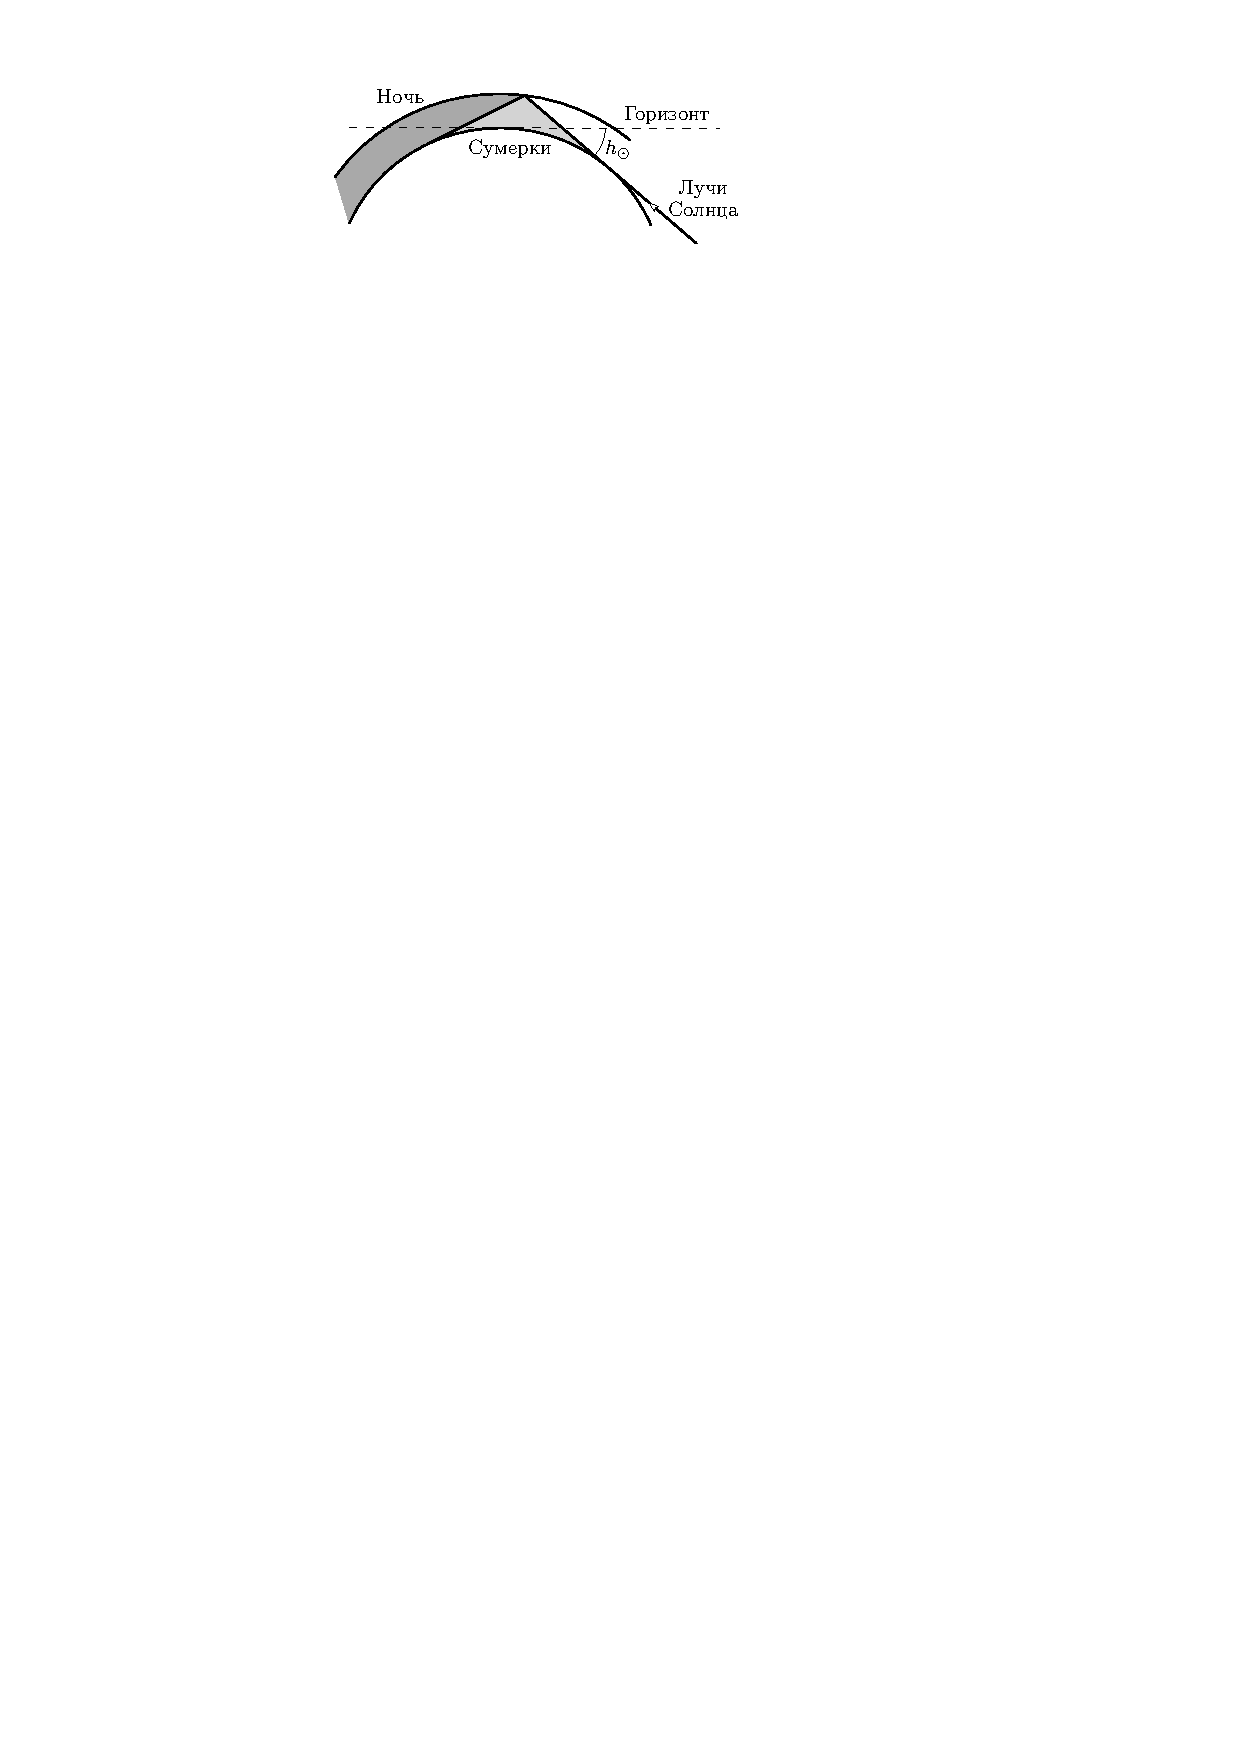
\includegraphics[width=\tw]{spher-astro-dusk.pdf}
	\captionof{figure}{Сумерки}
\end{minipage}
\newpage

